\documentclass[namedate,webpdf,traditional,large]{oup-authoring-template}

\usepackage{booktabs}
\usepackage{graphicx}
\usepackage{url}

\graphicspath{{Fig/}}
\newcommand{\societylogo}{}
\newcommand{\method}{RegionAdapterMoETCN}
\newcommand{\backbone}{RegionAwareTCN}
\newcommand{\twelve}{ESM2-t12}
\newcommand{\thirtythree}{ESM2-t33}
\newcommand{\placeholder}[1]{\textbf{[#1]}}

\begin{document}

\journaltitle{Bioinformatics}
\DOI{DOI added during production}
\copyrightyear{2026}
\pubyear{2026}
\vol{XX}
\issue{X}
\access{Published: Date added during production}
\appnotes{Original Paper}
\firstpage{1}

\title[Warm-start region adapters for IDR prediction]{\method: warm-start region-specialized adapters for calibrated sequence-only intrinsic disorder prediction}

\author[1,$\ast$]{\placeholder{First Author}}
\author[1]{\placeholder{Second Author}}
\author[2]{\placeholder{Senior Author}}

\address[1]{\orgdiv{\placeholder{Department}}, \orgname{\placeholder{Institution}}, \orgaddress{\street{\placeholder{Street}}, \postcode{\placeholder{Postcode}}, \state{\placeholder{State}}, \country{\placeholder{Country}}}}
\address[2]{\orgdiv{\placeholder{Department}}, \orgname{\placeholder{Institution}}, \orgaddress{\street{\placeholder{Street}}, \postcode{\placeholder{Postcode}}, \state{\placeholder{State}}, \country{\placeholder{Country}}}}

\corresp[$\ast$]{Corresponding author. \href{mailto:corresponding.author@example.edu}{corresponding.author@example.edu}}

%\received{Date}{0}{Year}
%\revised{Date}{0}{Year}
%\accepted{Date}{0}{Year}
%\editor{Associate Editor: Name}

\abstract{
\textbf{Motivation:} Intrinsic disorder prediction has benefited from protein language models, but benchmark gains remain difficult to interpret when disorder labels are regionally heterogeneous, test sets differ in prevalence, and homologous training examples may inflate apparent performance.\\
\textbf{Results:} We developed \method, a sequence-only residue-level predictor that warm-starts from an ESM2-t33 \backbone{} backbone and adds low-rank region-specialized adapters with a residue-level mixture-of-experts gate for short/long and terminal/internal disorder patterns. The final model uses three-seed score averaging, validation-selected thresholding and Platt calibration fitted only on the DM1229 validation set. Across SL329, MXD494 and DISORDER723, the P4.8 warm-start \method{} ensemble achieved AUC values of 0.920545, 0.850471 and 0.945409, respectively, exceeding curated direct state-of-the-art point AUC values under the full DM3000 training protocol. Relative to the P4.6 ESM2-t33 \backbone{} ensemble, the largest practical gain was observed on DISORDER723 internal IDRs, where AUC, AUPR and MCC improved by 0.007242, 0.019317 and 0.027346. Target-specific NR25 evaluation showed that warm-start adapters preserved low-homology robustness relative to P4.6 NR25 models. Platt calibration preserved ranking metrics while reducing DISORDER723 ECE from 0.159805 to 0.016327 and Brier score from 0.085060 to 0.032010.\\
\textbf{Availability:} Code, configuration files, reproducibility scripts, figures and manuscript assets will be available at \url{https://github.com/MedBio07/IDP_RegionAware}; trained model weights, prediction files and large derived artifacts will be archived with a permanent DOI before submission.\\
\textbf{Contact:} \href{mailto:corresponding.author@example.edu}{corresponding.author@example.edu}\\
\textbf{Supplementary information:} Supplementary data are available with the manuscript.
}

\keywords{intrinsic disorder prediction, intrinsically disordered regions, protein language model, ESM2, adapter, mixture of experts, calibration, uncertainty, low-homology evaluation}

\maketitle

\section{Introduction}

Intrinsically disordered proteins and intrinsically disordered regions (IDRs) are central to regulation, signaling, molecular recognition and protein interaction networks, yet their residue-level prediction remains a difficult sequence analysis problem \citep{wright1999intrinsically,necci2021caid}. Disorder is not a single homogeneous state. Disordered residues may occur in short or long segments, near the termini or inside proteins, and in proteins with very different overall disorder content. Benchmark labels also vary in origin and certainty, including DisProt-like annotations, missing-residue-derived annotations, NoX-style labels and unknown residues. These factors make global benchmark metrics useful but incomplete.

Recent intrinsic disorder predictors increasingly use protein language models (PLMs), feature fusion, ensembles and length-aware or region-aware training strategies \citep{tang2023idpfusion,pang2023idplm,nambiar2024drbert,xie2025idpedl,liu2025fusionencoder}. Community evaluations such as CAID have also shifted attention toward ranking metrics, threshold-dependent metrics, low-similarity subsets and disorder-function extensions \citep{necci2021caid,caid3_2026,pang2024disoflag}. Strong recent methods include IDP-EDL, which combines PLM representations with short-, long- and generic-disorder predictors, and FusionEncoder, which integrates traditional and PLM-based features through a fusion architecture \citep{xie2025idpedl,liu2025fusionencoder}. CAID-era methods such as PUNCH2, PredIDR2, DisorderUnetLM and flDPnn3 further show that PLM-based or hybrid representations are now central to competitive disorder prediction \citep{meng2025punch2,han2025predidr2,kotowski2025disorderunetlm,wang2026fldpnn3}.

Despite this progress, three issues remain important for a method paper. First, full-training benchmark gains can be misleading without explicit low-homology controls. Second, internal and terminal IDRs can have different error profiles that are hidden by aggregate AUC. Third, most predictors report raw scores rather than calibrated probabilities, limiting their practical use for experimental prioritization. In particular, a high residue-level score is more useful if it can be interpreted as a calibrated probability and accompanied by uncertainty information.

We present \method, a sequence-only residue-level IDR prediction framework that warm-starts from a strong ESM2-t33 \backbone{} model and adds low-rank region-specialized adapters with a learned residue-level mixture-of-experts gate \citep{lin2023esm,platt1999probabilistic}. The selected final model uses ESM2-t33-650M residue embeddings, one-hot and relative-position features, three-seed score averaging and validation-fitted Platt calibration. We keep the main model sequence-only and avoid PDB coordinates, experimentally missing residues, multiple-sequence alignments, profile features, AlphaFold confidence features and function labels as primary inputs. This design reduces leakage risk and simplifies deployment.

The study makes five contributions. First, it introduces a warm-start region-adapter MoE specialization over a strong sequence-only ESM2-t33 \backbone{} backbone. Second, it separates full DM3000 benchmark performance from target-specific NR25 low-homology training. Third, it reports hard-case stratification across short/long disorder, terminal/internal IDRs, residue zones and protein-level strata. Fourth, it fits Platt calibration on validation predictions and evaluates probability quality and uncertainty-error enrichment. Fifth, it includes exploratory gate analysis to test whether region routing is interpretable, while keeping the primary claim anchored to empirical benchmark, NR25 and hard-case evidence.

\section{Materials and Methods}

\subsection{Datasets and label handling}

The study used DM3000 as the training set and DM1229 as the validation set. Three independent external benchmarks were used for final testing: SL329, MXD494 and DISORDER723 (Table~\ref{tab:dataset}). Labels were treated at residue level with three states: ordered, disordered and unknown. Unknown residues were excluded from all metric calculations, which primarily affects SL329. Thresholds, calibration parameters and model choices were selected on DM1229 and fixed before test-set evaluation.

The three external benchmarks differ substantially in disorder prevalence. Among known residues, the disorder fraction is 0.435334 for SL329, 0.224360 for MXD494 and 0.062845 for DISORDER723. Because DISORDER723 is highly imbalanced, AUPR, MCC, Fmax and calibration metrics are reported alongside ROC-AUC.

\subsection{NR25 leakage-control evaluation}

Target-specific NR25 training sets were generated by removing DM3000 training proteins with MMseqs2 percentage identity above 25\% against each target benchmark \citep{steinegger2017mmseqs2}. The resulting training sets retained 2824 proteins for SL329, 2677 proteins for MXD494 and 2576 proteins for DISORDER723. Full DM3000 and NR25 results are reported separately to avoid mixing standard benchmark performance with low-homology generalization claims.

\subsection{Sequence representation and \method{}}

Residue-level ESM2 embeddings were extracted and cached. The P4.6 representation-upgrade experiment replaced ESM2-t12-35M layer 12 with ESM2-t33-650M layer 33 while keeping the \backbone{} temporal-convolutional head, thresholding protocol and benchmark evaluation fixed. This established the ESM2-t33 \backbone{} ensemble as the warm-start source and strongest internal baseline. \backbone{} applies temporal convolutional sequence modeling to frozen residue representations, residue one-hot features and relative-position features, with auxiliary supervision for short versus long disordered regions and terminal versus internal disorder patterns.

The P4.8 final predictor uses a warm-start adapter design. A shared temporal-convolutional backbone is initialized from a matched P4.6 ESM2-t33 \backbone{} checkpoint and then frozen. Four low-rank residual adapters and four expert heads correspond to SDR, LDR, terminal-IDR and internal-IDR patterns. A residue-level softmax gate mixes expert outputs and adds the resulting expert delta to a generic disorder logit. Only region adapters, expert heads and the gate head are trained during warm-start specialization. The final predictor averages scores from three independently warm-started seeds. The ensemble score is used for ranking metrics, validation-selected thresholding and calibration.

\subsection{Training, calibration and evaluation}

Models were trained on DM3000 or target-specific NR25 training sets and selected using validation performance on DM1229. The binary decision threshold was selected on DM1229 by maximizing Fmax for the corresponding score distribution. For the final full-training P4.8 Platt-calibrated ensemble, this validation-selected threshold was 0.331034 and was used for the Sn, Sp, BACC and MCC values reported in the main benchmark table. Test labels were never used for threshold tuning or calibration fitting.

Post-hoc calibration was fitted using DM1229 validation predictions. Raw scores, temperature scaling, Platt scaling and isotonic regression were evaluated. Platt scaling was selected for the main calibrated output because it preserved ranking metrics while improving expected calibration error (ECE), Brier score and negative log-likelihood with lower overfitting risk than isotonic regression. Uncertainty was computed from calibrated binary predictive entropy.

Residue-level performance was evaluated with sensitivity (Sn), specificity (Sp), balanced accuracy (BACC), Matthews correlation coefficient (MCC), ROC-AUC, AUPR and Fmax. Calibration quality was evaluated with ECE, Brier score and negative log-likelihood. Stratified analyses were performed for short disordered regions (SDRs), long disordered regions (LDRs), terminal/internal IDRs, residue zones, protein length bins and protein disorder-content bins. P4.8 \method{} and P4.6 \backbone{} predictions were compared with protein-level paired bootstrap confidence intervals and paired permutation tests. External SOTA methods were available only as aggregate published metrics, so they were compared as point references rather than by paired statistical tests. The mixture-of-experts gate was analyzed descriptively by averaging gate weights across the three warm-start seeds and summarizing them by region strata; this was treated as auxiliary mechanism evidence rather than a causal intervention.

\section{Results}

\subsection{Warm-start \method{} preserves full-benchmark performance and improves hard cases}

Under the full DM3000 training protocol, the P4.8 warm-start \method{} ensemble reached AUC values of 0.920545, 0.850471 and 0.945409 on SL329, MXD494 and DISORDER723, respectively (Table~\ref{tab:full}; Figure~\ref{fig:rocpr}). These point estimates exceed the curated direct SOTA AUC values for all three benchmarks: IDP-EDL on SL329, FusionEncoder on MXD494 and IDP-EDL on DISORDER723 \citep{xie2025idpedl,liu2025fusionencoder}. The corresponding point gaps versus SOTA were +0.005545, +0.008471 and +0.002409.

Compared with the P4.6 ESM2-t33 \backbone{} ensemble, P4.8 changed full-benchmark AUC by +0.001218 on SL329, -0.000166 on MXD494 and +0.000798 on DISORDER723. Protein-level bootstrap confidence intervals for the AUC delta were 0.000298 to 0.002092 on SL329, -0.001384 to 0.001085 on MXD494 and 0.000015 to 0.001502 on DISORDER723. Thus, the aggregate performance story is preservation with small favorable point changes, not large global dominance.

\subsection{Internal-IDR gains provide the strongest performance evidence}

The main practical improvement occurs in internal-IDR hard cases (Figure~\ref{fig:hardcase}; Table~\ref{tab:hardcase}). On DISORDER723 internal IDRs, P4.8 improved AUC from 0.887416 to 0.894658, AUPR from 0.152541 to 0.171858 and MCC from 0.210033 to 0.237379. DISORDER723 middle residues also improved, with AUC +0.001514, AUPR +0.010856 and MCC +0.007044. MXD494 internal-IDR MCC improved by 0.005448, although SL329 internal-IDR MCC decreased slightly. These results justify making internal-IDR behavior a central result while keeping dataset-specific caveats explicit.

This result connects to the prior failure analysis (Figure~\ref{fig:evidence}). Low-cost post-processing and loss variants did not close the DISORDER723 internal-IDR gap, and P4.6 showed that ESM2-t33 was the decisive representation upgrade. P4.8 then adds a smaller but more method-specific improvement by specializing the frozen P4.6 backbone with region adapters.

\subsection{NR25 evaluation defines the low-homology boundary}

Target-specific NR25 training reduced performance relative to full DM3000 training (Table~\ref{tab:nr25}). The P4.8 NR25 AUC values were 0.918557, 0.833695 and 0.938194 on SL329, MXD494 and DISORDER723. Relative to P4.6 NR25 baselines, the AUC deltas were +0.001496, -0.000394 and +0.001319. Under NR25 training, \method{} remained above the curated SL329 SOTA AUC but fell below the curated MXD494 and DISORDER723 SOTA AUC values. The appropriate claim is therefore robustness relative to the internal backbone baseline, not uniformly low-homology SOTA.

\subsection{Platt calibration improves probability quality and uncertainty tracks errors}

Platt calibration preserved AUC, AUPR and MCC while improving probability quality (Table~\ref{tab:calibration}). For the P4.8 model, ECE decreased from 0.108403 to 0.087562 on SL329, from 0.241887 to 0.108556 on MXD494 and from 0.159805 to 0.016327 on DISORDER723. Brier score decreased by 0.016725, 0.066280 and 0.053050, respectively.

Calibrated uncertainty was informative (Figure~\ref{fig:uncertainty}). The top 10\% most uncertain residues were enriched for errors by 2.73-fold on SL329, 2.52-fold on MXD494 and 7.03-fold on DISORDER723. This supports uncertainty-aware interpretation, especially for low-prevalence or annotation-sensitive benchmarks.

\subsection{Gate analysis supports only a cautious routing interpretation}

Exploratory gate analysis showed partial but not one-hot region specialization (Figure~\ref{fig:gate}). On DM1229 validation, SDR residues had mean SDR-gate weight 0.410476 and terminal-IDR residues had mean terminal-IDR-gate weight 0.433842. However, ordered validation residues had the highest mean internal-IDR gate component, and external internal-IDR routing was heterogeneous: internal target gate mass was 0.221655 on SL329, 0.239106 on MXD494 and 0.295357 on DISORDER723. The gate therefore should not be interpreted as a direct biological region classifier. It is better viewed as a learned routing mechanism that helps region-specific score correction after warm-starting.

\section{Discussion}

\method{} changes the manuscript emphasis from a representation-upgraded \backbone{} to a warm-start region-adapter specialization over a strong ESM2-t33 \backbone{} backbone. This matters for novelty: the main methodological claim is not simply that a larger PLM improves disorder prediction, but that a frozen strong backbone can be locally specialized with low-rank region adapters and a residue-level MoE gate while preserving calibration and low-homology robustness.

The claim boundary remains conservative. Full-benchmark AUC deltas over P4.6 are small, and paired permutation tests do not support broad global dominance. External SOTA methods do not provide residue-level predictions, so direct paired tests against them are not possible. The strongest direct evidence is the hard-case improvement on DISORDER723 internal IDRs, where AUC, AUPR and MCC all improve meaningfully. This gives the method a clearer biological and evaluation-centered rationale than aggregate AUC alone.

The NR25 experiments are a strength because they separate standard benchmark performance from low-homology generalization. P4.8 does not collapse under target-specific NR25 training and remains close to or slightly better than P4.6 NR25 baselines. However, MXD494 and DISORDER723 NR25 AUC values remain below curated external SOTA point values, so the paper should avoid claiming uniform low-homology SOTA.

Calibration is a practical contribution. Platt scaling markedly improves ECE and Brier score, especially on MXD494 and DISORDER723, without changing AUC, AUPR or MCC. Calibrated uncertainty also enriches prediction errors, supporting a caution signal for ambiguous residues, disorder boundaries and low-prevalence datasets.

The gate analysis is useful but limited. It shows routing shifts for validation SDR and terminal-IDR residues, yet it does not provide a clean biological decoder for every region type. This is not a failure of the model, but it constrains the interpretation: the gate should be framed as an optimization mechanism for region-specific adaptation, not as a stand-alone biological annotation model.

Internal IDRs remain the major unsolved technical problem. Although P4.8 improved DISORDER723 internal AUC, AUPR and MCC, internal-IDR classification remains difficult. This suggests that internal disorder may require additional signals, such as function-aware labels, binding-region annotations, molecular recognition feature labels or specialized hard-example training. Structure features should not be added casually because local audits found no controlled structure-feature coverage and several benchmarks contain PDB-chain-like identifiers, creating leakage risk. Structure-aware preprints and CAID3-era predictors should therefore be treated as important future-work context rather than as uncontrolled add-ons to the present sequence-only claim \citep{kabir2026esmdispred,wang2026fldpnn3}.

Overall, the strongest manuscript position is not that a new neural network solves IDR prediction. The stronger contribution is a transparent and calibrated PLM-era benchmark framework that preserves strong full-training performance, exposes low-homology and internal-IDR limitations, and shows that warm-start region adapters can improve the principal hard case without sacrificing calibration.

\section{Conclusion}

\method{} provides a sequence-only, warm-start region-adapter framework for residue-level intrinsic disorder prediction. The P4.8 three-seed ensemble achieves AUC-level SOTA point performance on three external benchmarks under the full DM3000 protocol, preserves target-specific NR25 robustness relative to P4.6, and provides its clearest practical improvement on DISORDER723 internal IDRs. Platt calibration substantially improves probability quality and calibrated uncertainty enriches prediction errors. The remaining limitations are small aggregate gains over the strong P4.6 backbone, heterogeneous gate interpretability, DISORDER723 MCC below external SOTA and non-uniform low-homology SOTA performance.

\section{Availability and implementation}

Code, configuration files, reproducibility scripts, figures and manuscript assets will be made available at \url{https://github.com/MedBio07/IDP_RegionAware}. Trained model weights, validation-fitted calibration parameters, residue-level predictions, benchmark result tables and large derived artifacts will be archived with a permanent DOI before submission. The local reproducibility package contains labeled FASTA datasets under \texttt{data/}, target-specific NR25 train-set construction artifacts under \texttt{data/nr25\_by\_test/}, cached ESM2 embeddings under \texttt{data/features/esm2\_embeddings/}, trained \method{} weights under \texttt{models/}, predictions under \texttt{predictions/}, result tables under \texttt{results/}, figures under \texttt{figures/}, and manuscript assets under \texttt{manuscript/}. The final public release should either include the cached ESM2 embeddings or provide exact commands for regenerating them from sequence FASTA files.

\section{Data availability}

The datasets, processed train/validation/test splits, prediction outputs, evaluation tables and manuscript figures will be released with the code repository subject to third-party dataset redistribution permissions. If direct redistribution of any benchmark file is restricted, the repository will provide construction scripts, checksums and instructions for obtaining the source data.

\section{Supplementary data}

Supplementary material includes the paper-level ablation table, protein-level bootstrap and paired permutation results, hard-case stratified performance, full calibration metrics and uncertainty-error enrichment tables.

\section{Funding}

\placeholder{Funding information to be filled before submission.}

\section{Conflict of interest}

\placeholder{Conflict of interest statement to be filled before submission.}

\section{Acknowledgements}

\placeholder{Acknowledgements to be filled before submission.}

\begin{figure*}[!t]
\centering
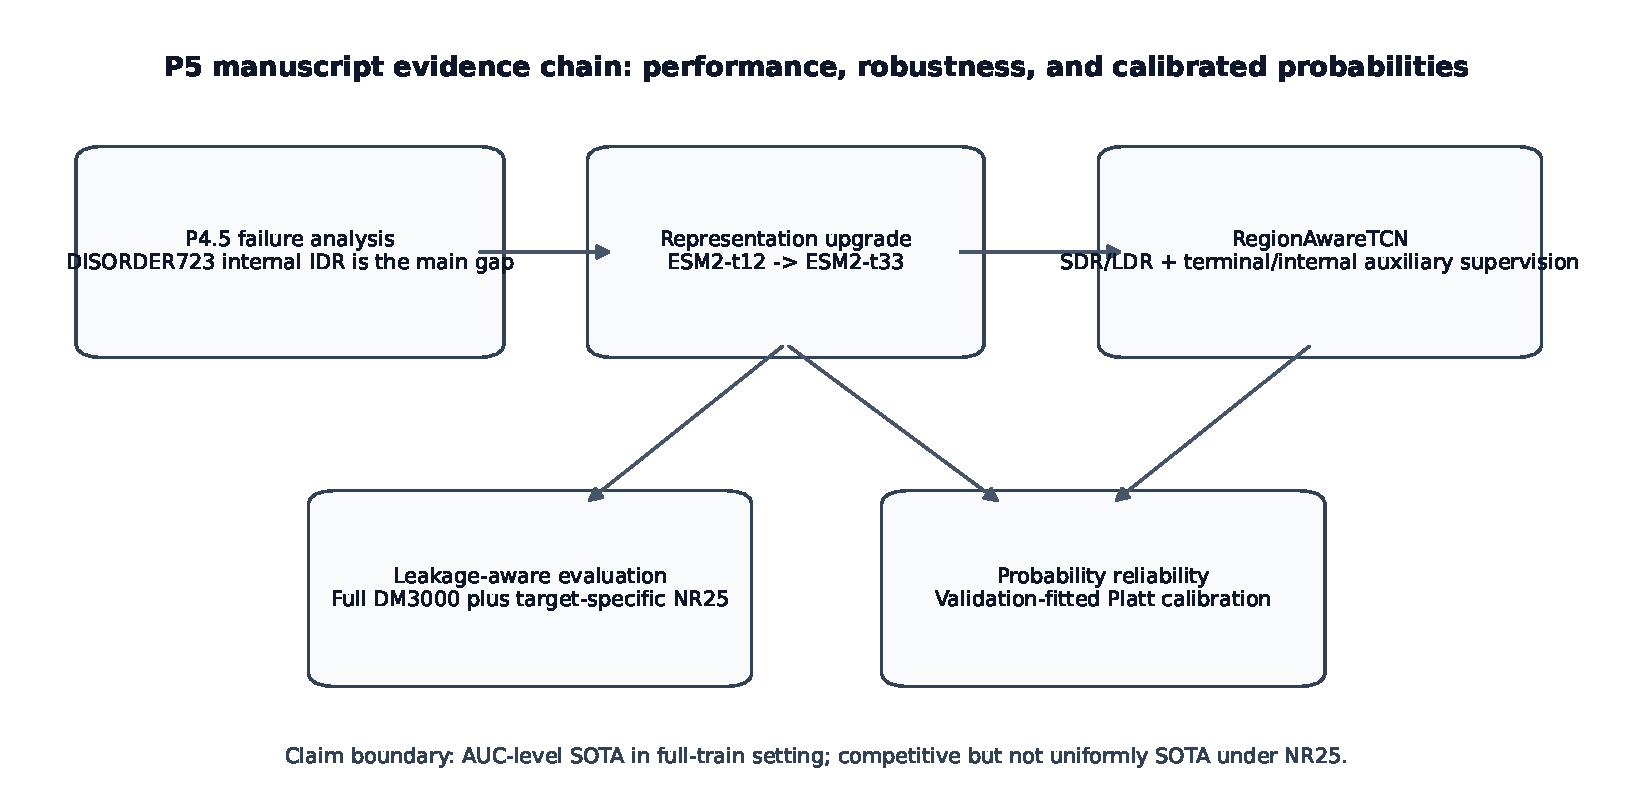
\includegraphics[width=\textwidth]{figure1_evidence_chain.pdf}
\caption{Evidence chain and model framing. The manuscript separates architecture choice, representation upgrading, calibration, NR25 robustness and hard-case analysis, keeping performance claims tied to their corresponding evidence level.}
\label{fig:evidence}
\end{figure*}

\begin{figure*}[!t]
\centering
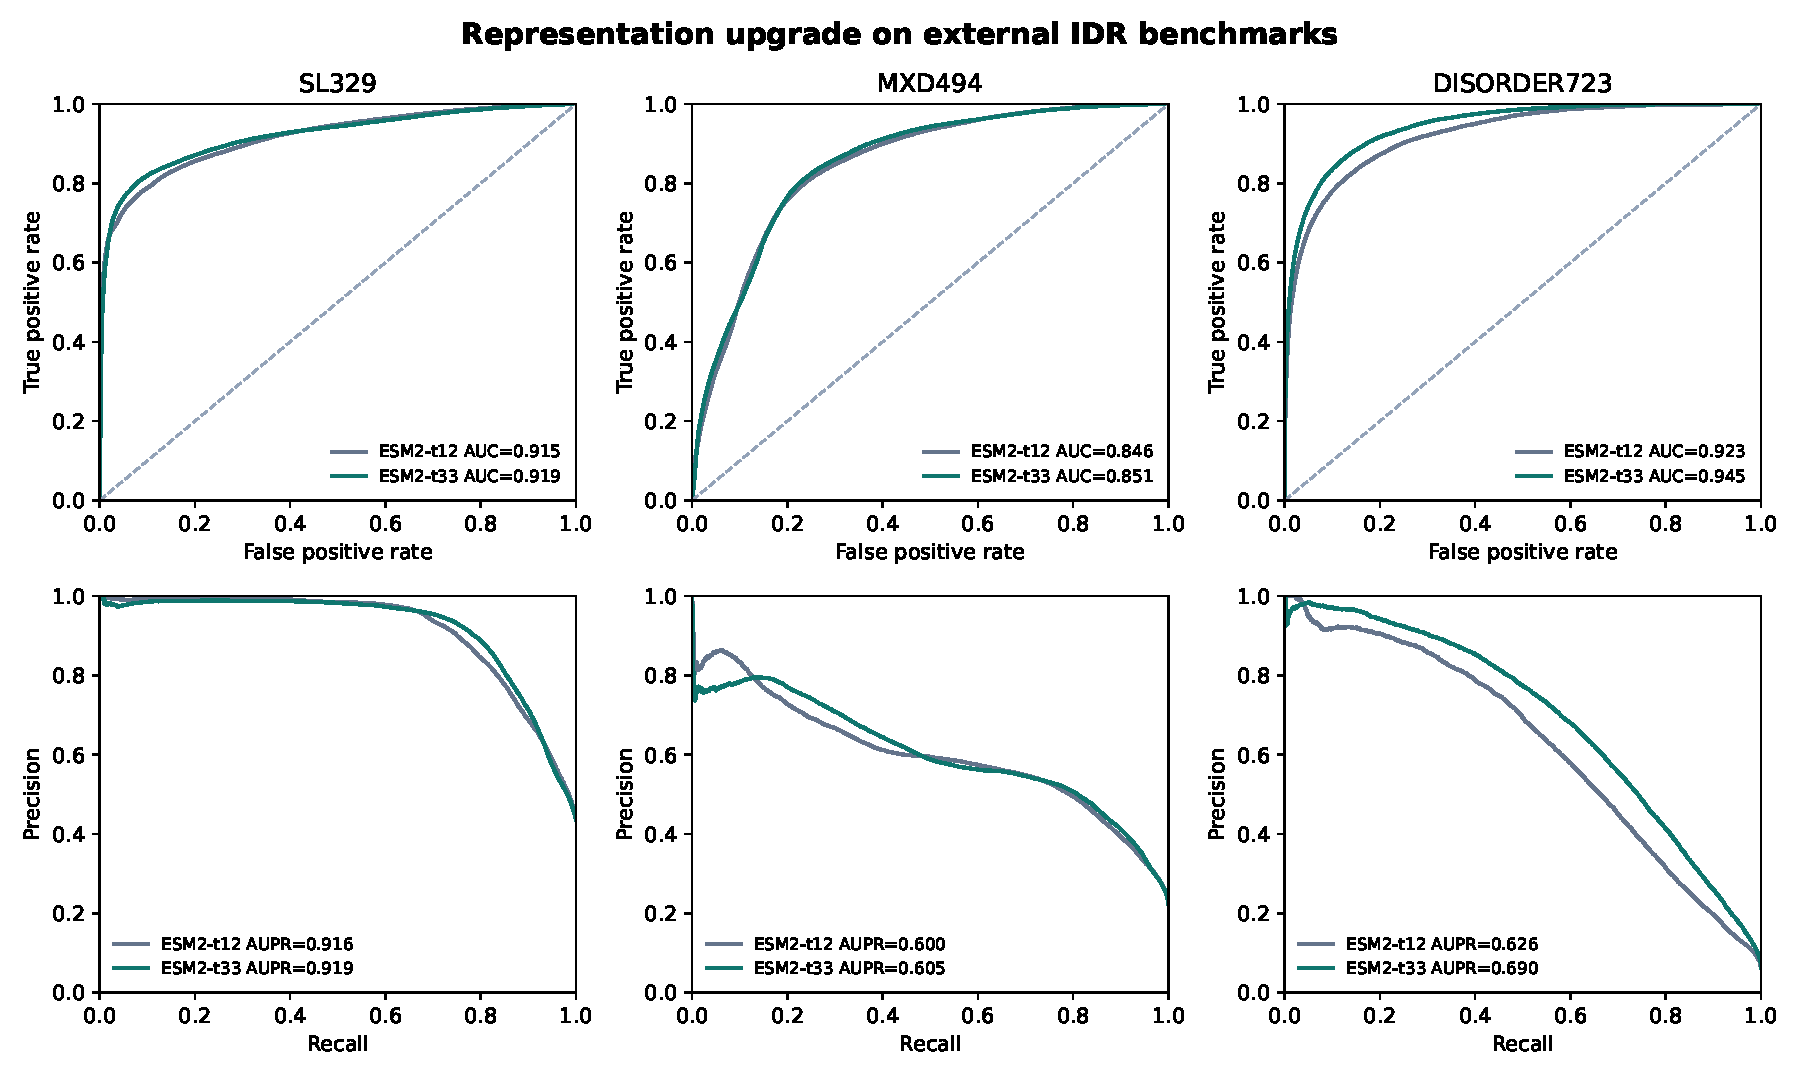
\includegraphics[width=\textwidth]{figure2_roc_pr.pdf}
\caption{ROC and precision-recall curves for the ESM2-t12 to ESM2-t33 representation upgrade. The largest and statistically supported AUC gain occurs on DISORDER723.}
\label{fig:rocpr}
\end{figure*}

\begin{figure*}[!t]
\centering
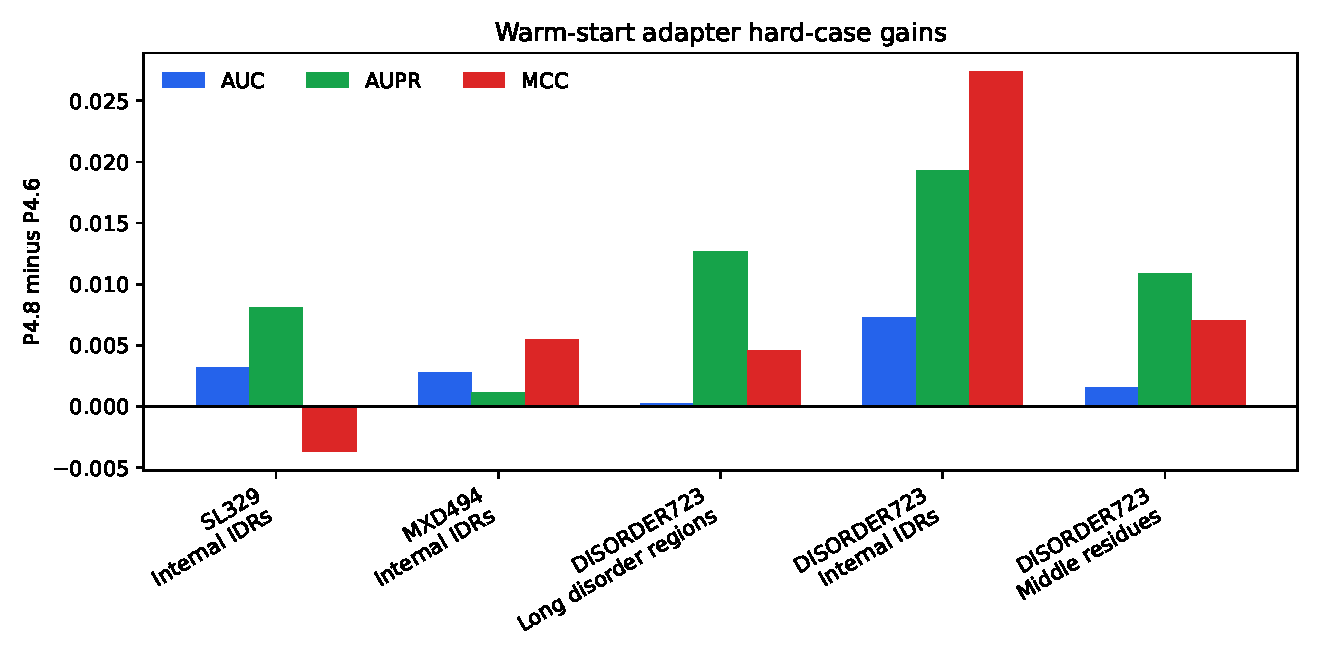
\includegraphics[width=\textwidth]{figure3_hard_case_gain.pdf}
\caption{Hard-case gains for the P4.8 warm-start \method{} ensemble relative to the P4.6 ESM2-t33 \backbone{} ensemble. The largest practical improvement occurs on DISORDER723 internal IDRs.}
\label{fig:hardcase}
\end{figure*}

\begin{figure*}[!t]
\centering
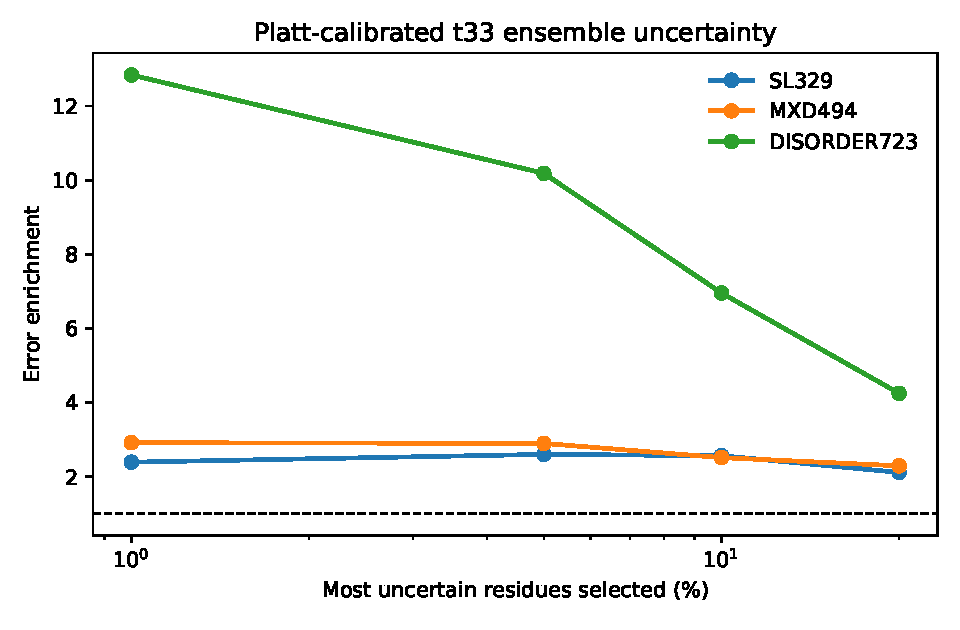
\includegraphics[width=\textwidth]{figure4_calibration_uncertainty.pdf}
\caption{Platt calibration and uncertainty-error enrichment. Calibrated uncertainty identifies error-enriched residues, especially on the highly imbalanced DISORDER723 benchmark.}
\label{fig:uncertainty}
\end{figure*}

\begin{figure*}[!t]
\centering
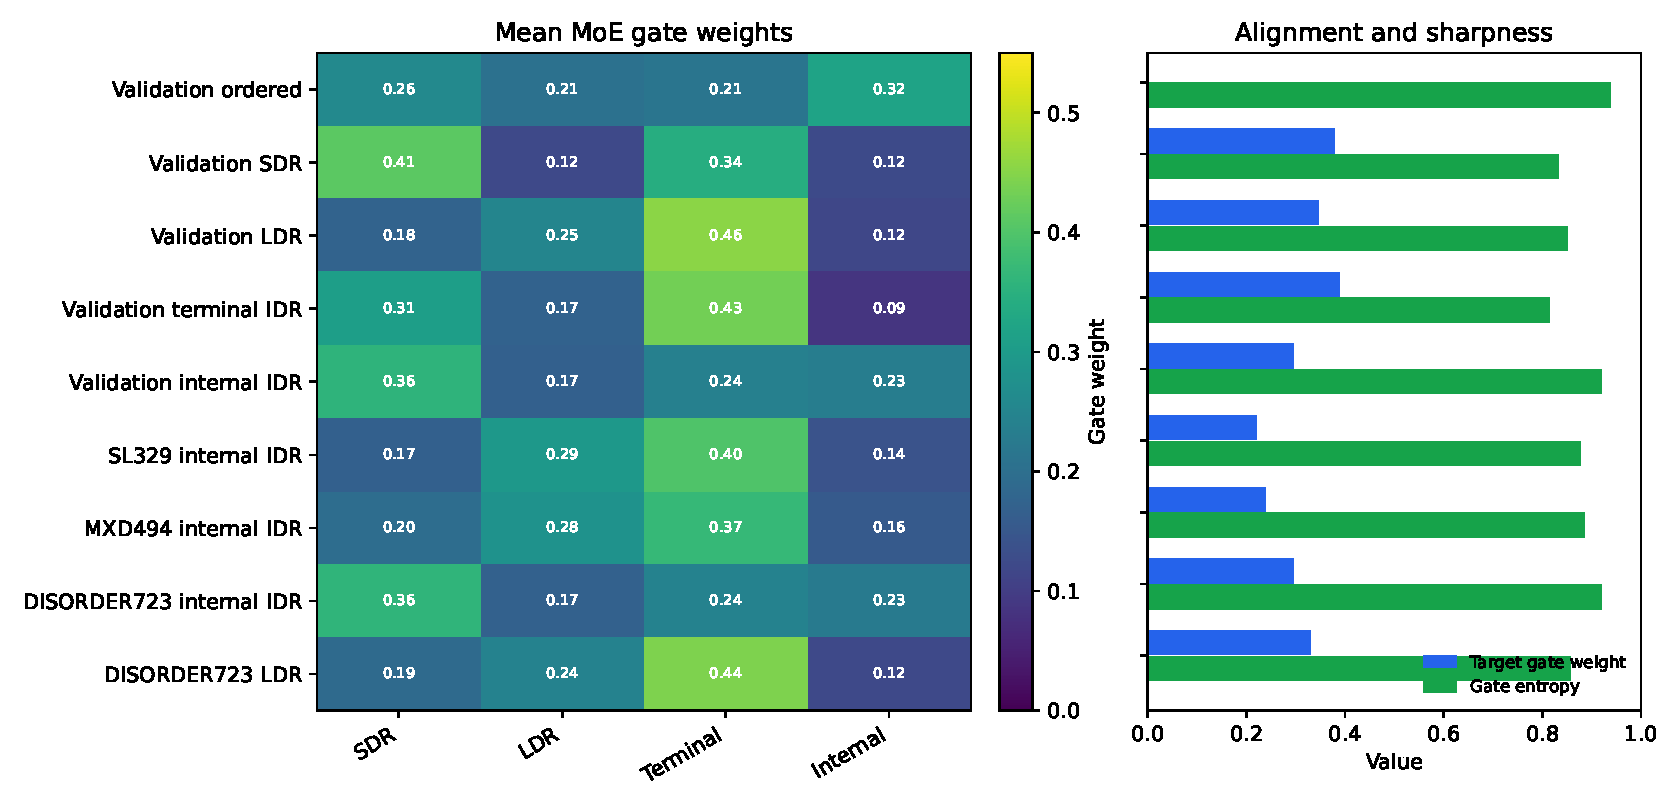
\includegraphics[width=\textwidth]{figure5_gate_specialization.pdf}
\caption{Exploratory MoE gate specialization analysis. Gate weights are partially aligned with validation SDR and terminal-IDR strata but are not clean one-hot biological region assignments; routing is therefore interpreted as an auxiliary score-specialization mechanism.}
\label{fig:gate}
\end{figure*}

\begin{table*}[!t]
\centering
\caption{Dataset and NR25 leakage-control summary. Unknown residues are masked during evaluation.}
\label{tab:dataset}
\scriptsize
\setlength{\tabcolsep}{3pt}
\begin{tabular}{lrrrrrrrrrr}
\toprule
Dataset & Proteins & Known & Disordered & Unknown & Disorder frac. & SDR & LDR & Terminal & Internal & NR25 kept \\
\midrule
DM3000 train & 3000 & 730804 & 74170 & 0 & 0.101491 & 5427 & 392 & 4183 & 1636 & NA \\
DM1229 validation & 1229 & 305830 & 29082 & 0 & 0.095092 & 2372 & 166 & 1751 & 787 & NA \\
SL329 test & 329 & 90836 & 39544 & 89582 & 0.435334 & 464 & 274 & 328 & 410 & 2824 \\
MXD494 test & 494 & 196501 & 44087 & 0 & 0.224360 & 577 & 271 & 517 & 331 & 2677 \\
DISORDER723 test & 723 & 215229 & 13526 & 0 & 0.062845 & 1363 & 60 & 1017 & 406 & 2576 \\
\bottomrule
\end{tabular}
\end{table*}

\begin{table*}[!t]
\centering
\caption{Full DM3000 benchmark performance for the P4.8 warm-start \method{} ensemble with Platt calibration. Binary metrics use the DM1229 validation-selected threshold. Paired statistics compare P4.8 against the P4.6 ESM2-t33 \backbone{} ensemble, not external aggregate SOTA methods.}
\label{tab:full}
\scriptsize
\setlength{\tabcolsep}{3pt}
\begin{tabular}{lrrrrrrrrrrr}
\toprule
Dataset & Sn & Sp & BACC & MCC & AUC & AUPR & Fmax & SOTA & SOTA AUC & P4.8-P4.6 AUC & P4.8-P4.6 MCC \\
\midrule
SL329 & 0.780902 & 0.935526 & 0.858214 & 0.733181 & 0.920545 & 0.920569 & 0.841076 & IDP-EDL & 0.915000 & 0.001218 & -0.003300 \\
MXD494 & 0.752104 & 0.807806 & 0.779955 & 0.501629 & 0.850471 & 0.602829 & 0.624979 & FusionEncoder & 0.842000 & -0.000166 & 0.002190 \\
DISORDER723 & 0.659175 & 0.972673 & 0.815924 & 0.613151 & 0.945409 & 0.693164 & 0.642751 & IDP-EDL & 0.943000 & 0.000798 & 0.002689 \\
\bottomrule
\end{tabular}
\end{table*}

\begin{table*}[!t]
\centering
\caption{Target-specific NR25 low-homology robustness. NR25 results are robustness evidence and are not uniformly SOTA.}
\label{tab:nr25}
\scriptsize
\setlength{\tabcolsep}{4pt}
\begin{tabular}{lrrrrrrrr}
\toprule
Dataset & Removed train & Kept train & Full AUC & NR25 AUC & NR25-full AUC & NR25 AUPR & Full MCC & NR25 MCC \\
\midrule
SL329 & 176 & 2824 & 0.920545 & 0.918557 & -0.001988 & 0.919279 & 0.733181 & 0.733606 \\
MXD494 & 323 & 2677 & 0.850471 & 0.833695 & -0.016776 & 0.590812 & 0.501629 & 0.483823 \\
DISORDER723 & 424 & 2576 & 0.945409 & 0.938194 & -0.007215 & 0.651359 & 0.613151 & 0.602456 \\
\bottomrule
\end{tabular}
\end{table*}

\begin{table*}[!t]
\centering
\caption{Hard-case gains of P4.8 \method{} over the P4.6 ESM2-t33 \backbone{} ensemble.}
\label{tab:hardcase}
\scriptsize
\setlength{\tabcolsep}{3pt}
\begin{tabular}{llrrrrrrrrr}
\toprule
Dataset & Stratum & Ref. AUC & P4.8 AUC & AUC delta & Ref. AUPR & P4.8 AUPR & AUPR delta & Ref. MCC & P4.8 MCC & MCC delta \\
\midrule
SL329 & Internal IDRs & 0.888676 & 0.891854 & 0.003178 & 0.733146 & 0.741248 & 0.008102 & 0.617910 & 0.614205 & -0.003705 \\
MXD494 & Internal IDRs & 0.796259 & 0.799026 & 0.002767 & 0.149714 & 0.150889 & 0.001175 & 0.228756 & 0.234204 & 0.005448 \\
DISORDER723 & LDR & 0.933028 & 0.933295 & 0.000267 & 0.498690 & 0.511333 & 0.012643 & 0.388454 & 0.393066 & 0.004612 \\
DISORDER723 & Internal IDRs & 0.887416 & 0.894658 & 0.007242 & 0.152541 & 0.171858 & 0.019317 & 0.210033 & 0.237379 & 0.027346 \\
DISORDER723 & Middle residues & 0.916962 & 0.918476 & 0.001514 & 0.443969 & 0.454825 & 0.010856 & 0.422864 & 0.429908 & 0.007044 \\
\bottomrule
\end{tabular}
\end{table*}

\begin{table*}[!t]
\centering
\caption{Platt calibration and uncertainty-error enrichment for the P4.8 warm-start \method{} ensemble. Calibration is fitted only on DM1229 validation predictions.}
\label{tab:calibration}
\scriptsize
\setlength{\tabcolsep}{4pt}
\begin{tabular}{lrrrrrrrrr}
\toprule
Dataset & AUC & AUPR & MCC & Raw ECE & Platt ECE & ECE delta & Raw Brier & Platt Brier & Top-10\% error enrich. \\
\midrule
SL329 & 0.920545 & 0.920569 & 0.733181 & 0.108403 & 0.087562 & -0.020841 & 0.125130 & 0.108405 & 2.730646 \\
MXD494 & 0.850471 & 0.602829 & 0.501629 & 0.241887 & 0.108556 & -0.133331 & 0.218987 & 0.152707 & 2.524622 \\
DISORDER723 & 0.945409 & 0.693164 & 0.613151 & 0.159805 & 0.016327 & -0.143478 & 0.085060 & 0.032010 & 7.028223 \\
\bottomrule
\end{tabular}
\end{table*}

\bibliographystyle{oup-abbrvnat}
\bibliography{regionawaretcn_refs}

\end{document}
